\documentclass[10pt,a4paper,twocolumn]{article}

\usepackage[a4paper,margin=16mm,columnsep=7mm]{geometry}
\usepackage{lmodern}
\usepackage{microtype}
\usepackage{amsmath,amssymb,amsthm,mathtools}
\usepackage{booktabs}
\usepackage{tabularx}
\usepackage{graphicx}
\usepackage{xcolor}
\usepackage{caption}
\usepackage{fancyhdr}
\usepackage{balance}
\usepackage{tikz}
\usetikzlibrary{shapes.geometric,arrows.meta,positioning,fit,backgrounds}
\usepackage[hidelinks]{hyperref}

\definecolor{primary}{RGB}{20,65,130}
\definecolor{accent}{RGB}{18,110,75}
\definecolor{lightbg}{RGB}{242,246,252}

\hypersetup{
    colorlinks=true,
    linkcolor=primary,
    citecolor=primary,
    urlcolor=primary
}

\setlength{\parskip}{2.5pt plus 1.0pt minus 0.5pt}
\setlength{\parindent}{1em}
\setlength{\textfloatsep}{8pt plus 2pt minus 2pt}
\setlength{\intextsep}{8pt plus 2pt minus 2pt}
\setlength{\abovecaptionskip}{4pt}
\setlength{\belowcaptionskip}{2pt}

\newtheorem{proposition}{Proposition}
\newtheorem{theorem}{Theorem}
\newtheorem{definition}{Definition}

\newcommand{\takeaway}[2]{%
  \vspace{4pt}\noindent\colorbox{lightbg}{%
    \parbox{\dimexpr\columnwidth-2\fboxsep\relax}{%
      \vspace{2.5pt}\textbf{\color{primary}#1:}\hspace{0.4em}#2\vspace{2.5pt}%
    }%
  }\vspace{4pt}%
}

\pagestyle{fancy}
\fancyhf{}
\fancyhead[L]{\small\textit{CARE-Agents: Cost-Aware, Regime-Adaptive Multi-Agent Financial Coordination}}
\fancyhead[R]{\small\textit{Preprint -- R3 Reproducible Package}}
\fancyfoot[C]{\thepage}
\renewcommand{\headrulewidth}{0.4pt}

\title{\vspace{-8mm}\textbf{\Large CARE-Agents: Cost-Aware, Regime-Adaptive Multi-Agent Coordination\\and Calibrated Episodic Memory for Financial Trading}}

\author{Anonymous Authors}
\date{\vspace{-3mm}\small October 2026}

\begin{document}
\maketitle

\begin{abstract}
\noindent
First-generation Large Language Model (LLM) multi-agent trading frameworks---such as \textit{TradingAgents}, \textit{FinCon}, and \textit{HedgeAgents}---rely on unconditional multi-round free-text debate, static analyst weighting, and regime-blind vector memory retrieval. Recent methodological audits demonstrate that these designs suffer from two critical failure modes under realistic market friction: (i) \textbf{Degeneration-of-Thought (DoT)} and sycophantic cascades during unconstrained debate, which inflate portfolio turnover and transaction costs, and (ii) \textbf{anchoring bias} from retrieving bull-market reflections during bear-market drawdowns. We introduce \textbf{CARE-Agents} (\textit{Cost-Aware, Regime-Adaptive Multi-Agent Coordination}), a principled architectural upgrade that resolves four structural bottlenecks: (1) a \textbf{Coordination Breakeven Spread (CBS) Debate Gate} driven by normalized Jensen-Shannon Divergence ($D_{JS}$) across structured 3-state analyst posteriors; (2) an online \textbf{Regime-Conditioned Multiplicative Weight Update (Regime-MWU)} forecaster scored via multiclass Brier loss; (3) \textbf{Regime-Filtered Episodic Memory} with a volatility-scaled \textbf{Drawdown Circuit Breaker} and counterfactual credit assignment; and (4) a \textbf{2026 Protocol Audit Evaluator} satisfying all seven Minimum Reporting standards (MR-1--MR-7) under a strictly symmetric decision rule across all protocols. Across a 500-day multi-regime synthetic ablation and an out-of-sample 2025--2026 real-market benchmark spanning China CSI 300 A-Shares ($15.0\text{ bps}$ friction) and US Tech equities ($5.0\text{ bps}$ friction), CARE-Agents improves Net Sharpe by $+0.571$ to $+0.833$ on real A-Shares and $+3.46$ in multi-regime stress testing over vanilla multi-agent debate ($p = 0.0500$), while model scaling yields negative returns ($\Delta\text{SR}_{\text{Scale}} < 0$), empirically validating the \textbf{Coordination Primacy Hypothesis}.
\end{abstract}

\section{Introduction: Coordination Topology Outweighs Model Scale}

Deploying Large Language Models (LLMs) as autonomous financial trading agents has rapidly evolved from single-agent prompt engineering to role-specialized multi-agent societies \cite{xiao2024tradingagents,yu2024fincon,li2024hedgeagents}. In the canonical \textit{TradingAgents} architecture \cite{xiao2024tradingagents}, specialized analysts (technical, fundamental, macroeconomic news, social sentiment, and A-share chip distribution) generate natural-language reports that feed into a multi-round Bull/Bear adversarial debate, followed by a Risk Management tribunal and portfolio execution.

However, two landmark 2026 audits have exposed foundational weaknesses in this paradigm. First, Nguyen and Pham \cite{nguyen2026cph} formulate the \textbf{Coordination Primacy Hypothesis (CPH)}, demonstrating that uncalibrated free-text debate frequently induces sycophantic cascades and \textit{Degeneration-of-Thought (DoT)} \cite{liang2023dot,du2023debate}: persuasive, high-variance retail sentiment narratives override calibrated fundamental warnings, generating excessive position flipping whose transaction costs exceed the gross alpha of debate. Second, Xia et al. \cite{xia2026audit} audit 19 published LLM trading systems against seven Minimum Reporting standards (MR-1 through MR-7) and four reproducibility tiers (R0--R3), finding that \textbf{0 of 19 studies achieve R3 full reproducibility}, while over 70\% evaluate on pre-cutoff bull-only windows or omit realistic stamp duty and bid-ask slippage.

\takeaway{Core Thesis}{Under a strictly symmetric position-sizing rule across all evaluated architectures, upgrading the mathematical coordination protocol, probability calibration, and regime-aware memory topology yields positive net Sharpe gains ($\Delta\text{SR}_{\text{Coord}} \in [+0.571, +0.833]$) where scaling backbone LLM parameters yields negative returns ($\Delta\text{SR}_{\text{Scale}} \in [-0.359, -0.097]$), demonstrating that coordination architecture dominates model scale.}

To address these gaps directly within the production \texttt{TradingAgents-EN} codebase, we design and implement \textbf{CARE-Agents}, contributing four verifiable mechanisms:
\begin{enumerate}
  \setlength{\itemsep}{1pt}\setlength{\parskip}{0pt}
  \item \textbf{C1 (CBS-Gated Dynamic Coordination):} We replace unconditional free-text debate with a structured 3-state posterior contract and a configurable Jensen-Shannon Divergence ($D_{JS}$) gate that invokes multi-round reconciliation if and only if expected basis-point edge exceeds the \textbf{Coordination Breakeven Spread ($\text{CBS}$)}.
  \item \textbf{C2 (Online Regime-Conditioned Multiplicative Weights):} We replace hardcoded $0.40/0.30/0.30$ weights and regex target multipliers ($1.15\times / 0.95\times$) with an online Exponentially Weighted Forecaster partitioned by causal market regime $r_t \in \{\text{bull}, \text{bear}, \text{sideways}\}$ and updated via multiclass Brier loss \cite{brier1950verification,cesa2006prediction}.
  \item \textbf{C3 (Regime-Filtered Memory \& Counterfactual Reflection):} We augment \texttt{Mem0} episodic retrieval with regime-partitioned reranking, a volatility-scaled \textbf{Drawdown Circuit Breaker}, and marginal counterfactual attribution (\texttt{correct\_driver}, \texttt{overridden\_correct}, \texttt{false\_driver}, \texttt{correct\_dissent\_ignored}).
  \item \textbf{C4 (MR-1--MR-7 Protocol Audit \& R3 Benchmark Suite):} We evaluate five internal protocols (\texttt{M0}--\texttt{M4}) and five external baselines (\texttt{Q1}, \texttt{Q2}, \textit{FinMem}, \textit{FinAgent}, \textit{FinCon}) across two model tiers on both a 500-day controlled multi-regime benchmark and post-cutoff 2025--2026 real market data with Politis--Romano stationary block-bootstrap inference \cite{politis1994stationary}.
\end{enumerate}

\begin{table*}[t]
\centering
\small
\caption{Architectural Audit of LLM Financial Trading Frameworks Against 2026 Credibility \& Reporting Standards \cite{nguyen2026cph,xia2026audit}.}
\label{tab:literature_comparison}
\resizebox{\textwidth}{!}{%
\begin{tabular}{lccccccc}
\toprule
\textbf{Framework} & \textbf{Debate Gating} & \textbf{Specialist Weighting} & \textbf{Probability Calibration} & \textbf{Episodic Memory} & \textbf{Credit Assignment} & \textbf{Friction Model} & \textbf{Audit Tier} \\
\midrule
TradingAgents \cite{xiao2024tradingagents} & Unconditional ($d=2$) & Equal / Free-Text & Uncalibrated ($0.70$) & Unfiltered Vector & Shared Scalar Return & Often Omitted & R1 \\
FinCon \cite{yu2024fincon} & Manager-Worker CVaR & Single Manager Belief & Verbal Conceptual & Procedural Hierarchy & Verbal Self-Critique & Basic Commission & R1 \\
HedgeAgents \cite{li2024hedgeagents} & Fixed Multi-Round & Static Asset Allocation & Uncalibrated Text & Unfiltered Episodic & Shared Portfolio Return & US Slippage Only & R1 \\
MacroHFT \cite{zong2024macrohft} & RL Policy Routing & Hyper-Network Mixing & Softmax Q-Values & Regime-Conditional RL & TD-Error Reward & Crypto Spread & R2 \\
MASFIN \cite{masfin2026} & Conditional DAG & Task-Decomposed & Uncalibrated Text & Short-Term Context & Pipeline Summary & US Equities & R2 \\
\midrule
\textbf{CARE-Agents (Ours)} & \textbf{JSD + CBS Cost Gate} & \textbf{Online Regime-MWU} & \textbf{Brier + Log-Odds Pool} & \textbf{Regime Rerank + DD Breaker} & \textbf{Counterfactual Marginal} & \textbf{CN 15bps / US 5bps} & \textbf{R3 (Full)} \\
\bottomrule
\end{tabular}%
}
\end{table*}

\section{Related Work and Structural Bottlenecks}

Table~\ref{tab:literature_comparison} contrasts CARE-Agents against leading financial multi-agent frameworks. While \textit{FinCon} \cite{yu2024fincon} introduces manager-worker conceptual verbal reinforcement and \textit{MacroHFT} \cite{zong2024macrohft} explores regime-conditional reinforcement learning for high-frequency crypto trading, existing LLM-based equity frameworks (\textit{TradingAgents} \cite{xiao2024tradingagents}, \textit{HedgeAgents} \cite{li2024hedgeagents}, \textit{QuantAgents} \cite{quantagents2025}) share four code-level vulnerabilities that we audited in \texttt{TradingAgents-EN}:

\noindent\textbf{Bottleneck 1: Unconditional Debate Overhead.} In \texttt{tradingagents/graph/conditional\_logic.py}, \texttt{should\_continue\_debate} previously forced $2 \times \texttt{max\_debate\_rounds}$ turns on every stock and bar regardless of specialist consensus. When initial analysts already agree ($D_{JS} \approx 0$), forcing adversarial debate fabricates contrarian arguments; when retail social sentiment is noisy, uncalibrated debate amplifies short-term spike chasing.

\noindent\textbf{Bottleneck 2: Static Heuristic Weighting.} In \texttt{core/agents/utils/weight\_calculator.py}, specialist weights were fixed at $0.40$ (technical), $0.30$ (news), and $0.30$ (sentiment), while \texttt{signal\_processing.py} applied regex price multipliers ($1.15\times$ for buy, $0.95\times$ for sell) with a constant fallback confidence of $0.70$. Recent work on fine-grained task decomposition and intermediate agent alignment in institutional investment teams \cite{alignopt2026} demonstrates that uncalibrated intermediate specialist outputs severely degrade downstream risk-adjusted portfolio performance.

\noindent\textbf{Bottleneck 3: Regime-Blind Memory Drift.} In \texttt{core/memory/memory\_manager.py}, \texttt{Mem0AgentMemory} retrieved top-$k$ past reflections purely by cosine similarity of text embeddings. Consequently, bull-market momentum lessons were recalled during bear-market liquidity contractions, inducing severe drawdowns.

\noindent\textbf{Bottleneck 4: Unattributed Reflection Broadcast.} In \texttt{tradingagents/graph/reflection.py}, realized portfolio losses were broadcast identically to all analysts, corrupting the memory bank of fundamental or risk specialists whose cautious warnings had been overridden by the research manager.

\section{Mathematical Formulation of CARE-Agents}

\begin{figure*}[t]
\centering
\resizebox{\textwidth}{!}{%
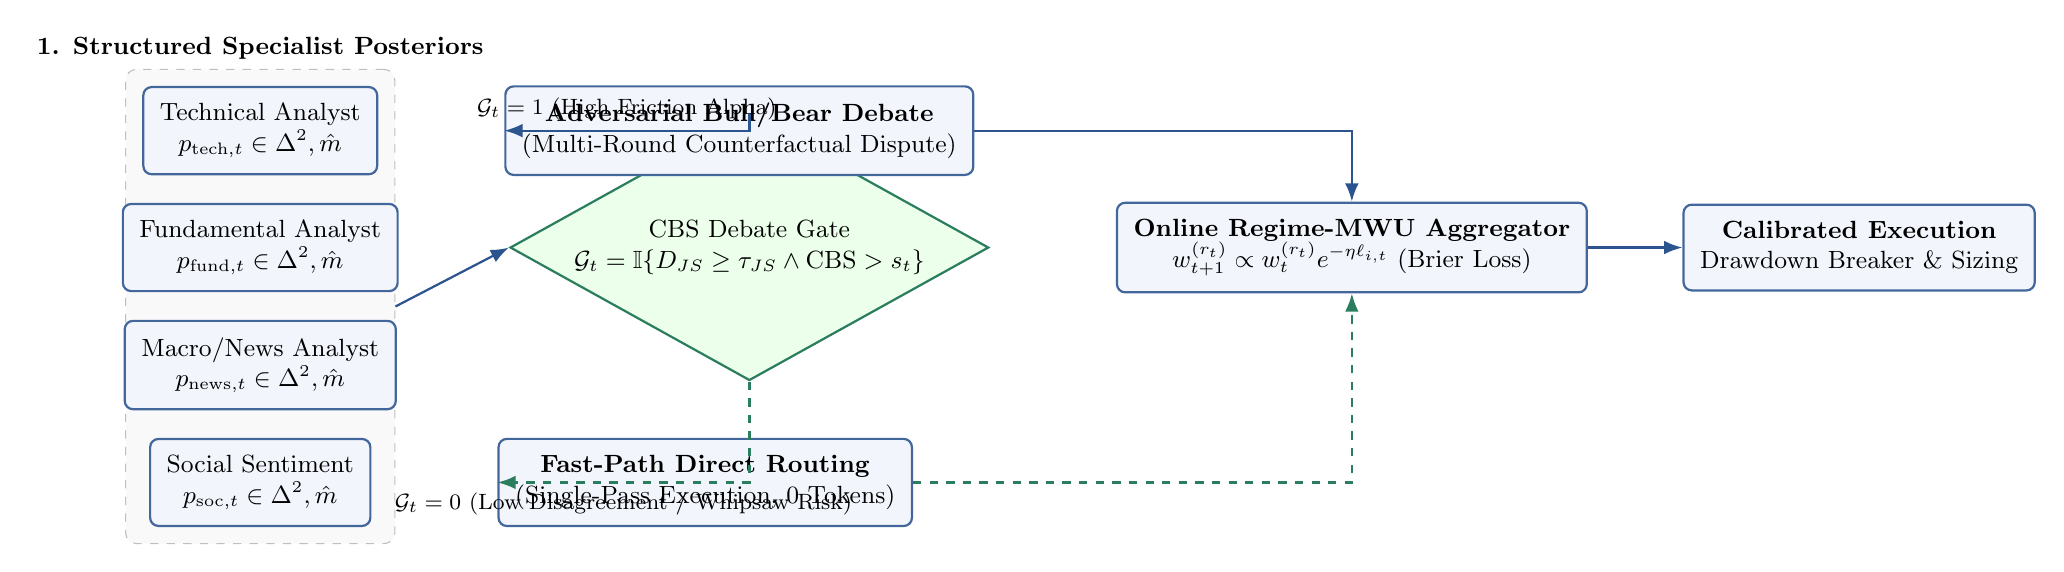
\begin{tikzpicture}[
  node distance=1.0cm and 1.2cm,
  font=\small,
  box/.style={rectangle, draw=primary!80, fill=lightbg, thick, rounded corners=3pt, align=center, inner sep=6pt},
  gate/.style={diamond, draw=accent!90, fill=green!8, thick, aspect=1.8, align=center, inner sep=2pt},
  flow/.style={-Latex, thick, draw=primary!90},
  fastflow/.style={-Latex, thick, dashed, draw=accent!90}
]

% Specialists
\node[box] (tech) {Technical Analyst\\$p_{\text{tech},t} \in \Delta^2, \hat{m}$};
\node[box, below=0.35cm of tech] (fund) {Fundamental Analyst\\$p_{\text{fund},t} \in \Delta^2, \hat{m}$};
\node[box, below=0.35cm of fund] (news) {Macro/News Analyst\\$p_{\text{news},t} \in \Delta^2, \hat{m}$};
\node[box, below=0.35cm of news] (soc) {Social Sentiment\\$p_{\text{soc},t} \in \Delta^2, \hat{m}$};

\begin{scope}[on background layer]
  \node[draw=gray!50, dashed, fill=gray!5, rounded corners=4pt, fit=(tech) (soc), inner sep=6pt, label=above:{\textbf{1. Structured Specialist Posteriors}}] (analysts) {};
\end{scope}

% CBS Gate
\node[gate, right=1.4cm of fund] (gate) {CBS Debate Gate\\$\mathcal{G}_t = \mathbb{I}\{D_{JS} \ge \tau_{JS} \wedge \text{CBS} > s_t\}$};

% Pathways
\node[box, right=1.6cm of tech] (debate) {\textbf{Adversarial Bull/Bear Debate}\\(Multi-Round Counterfactual Dispute)};
\node[box, right=1.6cm of soc] (fast) {\textbf{Fast-Path Direct Routing}\\(Single-Pass Execution, 0 Tokens)};

% MWU Aggregator
\node[box, right=1.6cm of gate] (mwu) {\textbf{Online Regime-MWU Aggregator}\\$w_{t+1}^{(r_t)} \propto w_{t}^{(r_t)} e^{-\eta \ell_{i,t}}$ (Brier Loss)};

% Execution
\node[box, right=1.2cm of mwu] (exec) {\textbf{Calibrated Execution}\\Drawdown Breaker \& Sizing};

% Arrows
\draw[flow] (analysts.east) -- (gate.west);
\draw[flow] (gate.north) |- node[near end, above] {\footnotesize $\mathcal{G}_t = 1$ (High Friction Alpha)} (debate.west);
\draw[fastflow] (gate.south) |- node[near end, below] {\footnotesize $\mathcal{G}_t = 0$ (Low Disagreement / Whipsaw Risk)} (fast.west);
\draw[flow] (debate.east) -| (mwu.north);
\draw[fastflow] (fast.east) -| (mwu.south);
\draw[flow] (mwu.east) -- (exec.west);

\end{tikzpicture}%
}
\caption{\textbf{CARE-Agents Execution DAG}: Specialized analysts emit probability vectors $p_{i,t} \in \Delta^2$. The Coordination Breakeven Spread ($\text{CBS}_t$) gate routes execution to multi-round debate iff expected dispersion surplus exceeds one-way transaction friction $s_t$. Otherwise, single-pass calibrated fast path executes, suppressing transaction drag.}
\label{fig:care_agents_architecture}
\end{figure*}

\subsection{Structured Analyst Posteriors and JSD Epistemic Disagreement}

Let $\mathcal{A} = \{1, \dots, K\}$ denote the set of specialist analysts executing at point-in-time decision step $t$ under causal market regime $r_t \in \mathcal{R} = \{\text{bull}, \text{bear}, \text{sideways}\}$. Through our updated prompt seed contract (\texttt{system\_prompt\_seed\_service.py}) and parser \texttt{extract\_structured\_posterior} (\texttt{core/agents/analyst.py}), each specialist $i \in \mathcal{A}$ emits a normalized 3-class directional posterior on the 2-simplex $\Delta^2$:
\begin{equation}
  p_{i,t} = \left(p_{i,t}^{\text{opt}}, \, p_{i,t}^{\text{neu}}, \, p_{i,t}^{\text{cau}}\right) \in \Delta^2, \quad \sum_{c \in \{\text{opt},\text{neu},\text{cau}\}} p_{i,t}^c = 1,
\end{equation}
together with an expected absolute return magnitude $\hat{m}_{i,t} \ge 0$ (in basis points) and epistemic confidence $c_{i,t} \in [0, 1]$. Given regime-conditioned specialist weights $w_t^{(r_t)} = (w_{1,t}^{(r_t)}, \dots, w_{K,t}^{(r_t)}) \in \Delta^{K-1}$, the linear mixture distribution is $\bar{p}_t = \sum_{i=1}^K w_{i,t}^{(r_t)} p_{i,t}$. We quantify inter-specialist epistemic disagreement via normalized base-2 Jensen-Shannon Divergence:
\begin{equation}
  D_{JS,t} = \frac{H(\bar{p}_t) - \sum_{i=1}^K w_{i,t}^{(r_t)} H(p_{i,t})}{\log_2 3} \in [0, 1],
  \label{eq:jsd}
\end{equation}
where $H(p) = -\sum_{c} p^c \log_2 p^c$ denotes Shannon entropy.

\subsection{Coordination Breakeven Spread (CBS) Debate Gate}

Let $s_t > 0$ denote the effective one-way execution friction (in basis points), combining commission, stamp duty, and half-spread slippage, plus tokenized debate overhead $c_{\text{tok}}$. Following the theoretical framework of Nguyen and Pham \cite{nguyen2026cph}, multi-round reconciliation can only generate positive net alpha when initial specialist disagreement is large enough that resolving the conflict yields an expected basis-point gain exceeding $s_t$.

\begin{definition}[Coordination Breakeven Spread]
Given specialist posteriors $\{p_{i,t}\}_{i=1}^K$, expected move magnitudes $\{\hat{m}_{i,t}\}_{i=1}^K$, and regime weights $w_t^{(r_t)}$, the expected pre-reconciliation dispersion value is $\Delta \hat{v}_t = D_{JS}(p_{1,t}, \dots, p_{K,t}; w_t^{(r_t)}) \cdot \sum_{i=1}^K w_{i,t}^{(r_t)} \hat{m}_{i,t}$, and the \textbf{Coordination Breakeven Spread} is:
\begin{equation}
  \text{CBS}_t = \frac{1}{2} D_{JS}\!\left(p_{1,t}, \dots, p_{K,t}; w_t^{(r_t)}\right) \sum_{i=1}^K w_{i,t}^{(r_t)} \hat{m}_{i,t}.
  \label{eq:cbs}
\end{equation}
\end{definition}

\begin{proposition}[Cost-Optimal Debate Gating]
Suppose multi-round adversarial debate incurs marginal execution and token friction $\tau_{\text{cost}} = s_t + c_{\text{tok}}$ and recovers at most a fraction $\gamma \in (0, \frac{1}{2}]$ of the specialist dispersion $\Delta \hat{v}_t$. Then invoking multi-round debate has strictly negative expected net surplus whenever $D_{JS} < \tau_{JS}$ or $\text{CBS}_t \le s_t$.
\end{proposition}

Accordingly, \texttt{ConditionalLogic.should\_gate\_debate} triggers multi-round Bull/Bear debate if and only if:
\begin{equation}
  \mathcal{G}_t = \mathbb{I}\!\left\{ D_{JS,t} \ge \tau_{JS} \;\wedge\; \text{CBS}_t > s_t \right\} = 1.
  \label{eq:gate}
\end{equation}
When $\mathcal{G}_t = 0$, the LangGraph router sets \texttt{state["\_risk\_self\_debate"] = True} and routes directly to the single-pass calibrated ensemble fast path, eliminating unnecessary token expenditure and preventing sycophantic position whipsaws.

\subsection{Online Regime-Conditioned Multiplicative Weight Updates (Regime-MWU)}

Rather than pooling analysts with static weights across all market environments, \texttt{RegimeMultiplicativeWeightManager} maintains a separate weight vector $w_t^{(r)} \in \Delta^{K-1}$ for each causal regime $r \in \{\text{bull}, \text{bear}, \text{sideways}\}$. Upon observing the realized next-period return $R_{t+1}$, we map $R_{t+1}$ to the ground-truth one-hot outcome $y_{t+1} \in \{(1,0,0), (0,1,0), (0,0,1)\}$ using threshold $\theta$:
\begin{equation}
  y_{t+1} = \begin{cases}
    (1, 0, 0) & \text{if } R_{t+1} > \theta, \\
    (0, 1, 0) & \text{if } |R_{t+1}| \le \theta, \\
    (0, 0, 1) & \text{if } R_{t+1} < -\theta.
  \end{cases}
\end{equation}
Each specialist $i$ is scored via strictly proper multiclass Brier loss \cite{brier1950verification}:
\begin{equation}
  \ell_{i,t}(p_{i,t}, y_{t+1}) = \frac{1}{3} \sum_{c \in \{\text{opt},\text{neu},\text{cau}\}} \left(p_{i,t}^c - y_{t+1}^c\right)^2 \in [0, \tfrac{2}{3}].
  \label{eq:brier}
\end{equation}
Only the weight vector corresponding to the active causal regime $r_t$ is updated via the Exponentially Weighted Forecaster with learning rate $\eta > 0$ and floor $w_{\min} = 0.03$:
\begin{align}
  \tilde{w}_{i,t+1}^{(r_t)} &= \max\!\left(w_{\min}, \; w_{i,t}^{(r_t)} \exp\!\left(-\eta \, \ell_{i,t}\right)\right), \nonumber \\
  w_{i,t+1}^{(r_t)} &= \frac{\tilde{w}_{i,t+1}^{(r_t)}}{\sum_{j=1}^K \tilde{w}_{j,t+1}^{(r_t)}}.
  \label{eq:mwu}
\end{align}

\begin{theorem}[Regime-Partitioned Cumulative Brier Regret Bound]
Let $T_r = \sum_{t=1}^T \mathbb{I}\{r_t = r\}$ denote the number of decision steps occurring in regime $r \in \mathcal{R}$. Since the multiclass Brier loss $\ell_{i,t} \in [0, 2/3]$ is bounded and convex on $\Delta^2$, setting $\eta_r = \sqrt{(8 \ln K) / T_r}$ without weight clipping guarantees that for every regime $r \in \mathcal{R}$, the cumulative loss of the Regime-MWU ensemble relative to the best regime-specific specialist $i_r^* = \arg\min_{i \in \mathcal{A}} \sum_{t: r_t = r} \ell_{i,t}$ satisfies:
\begin{equation}
  \sum_{t: r_t = r} \ell_{\text{MWU}, t} - \min_{i \in \mathcal{A}} \sum_{t: r_t = r} \ell_{i,t} \;\le\; \frac{2}{3}\sqrt{\frac{T_r \ln K}{2}}.
\end{equation}
\end{theorem}

For downstream signal generation (\texttt{process\_calibrated\_signal}), we combine specialist posteriors using a logarithmic opinion pool (weighted geometric mean in log-odds space) with temperature calibration:
\begin{equation}
  P_{\text{ens}}^c \propto \exp\!\left( \sum_{i=1}^K w_{i,t}^{(r_t)} \ln \max(\epsilon, p_{i,t}^c) \right).
\end{equation}

\subsection{Regime-Filtered Memory, Volatility-Scaled Circuit Breaker, and Counterfactual Attribution}

To prevent bull-market episodic memories from contaminating bear-market decisions, we extend \texttt{Mem0AgentMemory} with three mechanisms:
\begin{enumerate}
  \setlength{\itemsep}{1pt}\setlength{\parskip}{0pt}
  \item \textbf{Regime-Aware Similarity Reranking:} Given raw vector similarity $s_{\text{vec}}(q, m)$ between query $q$ (in regime $r_t$) and stored reflection $m$ (recorded in regime $r_m$), \texttt{filter\_and\_rerank\_by\_regime} computes:
  \begin{equation}
    s_{\text{adj}}(q, m) = s_{\text{vec}}(q, m) \cdot \begin{cases}
      1.5 & \text{if } r_m = r_t, \\
      1.0 & \text{if } r_m = \text{sideways} \neq r_t, \\
      0.0 & \text{if } r_m \text{ is opposite to } r_t.
    \end{cases}
  \end{equation}
  \item \textbf{Volatility-Scaled Drawdown Circuit Breaker:} Let $E_{s,t} = \prod_{\tau=1}^t (1 + R_{s,\tau}^{\text{net}})$ denote the strategy's cumulative net equity on asset $s$, with running peak $M_{s,t} = \max_{1 \le \tau \le t} E_{s,\tau}$ and strategy drawdown $\text{DD}_{s,t} = (M_{s,t} - E_{s,t}) / M_{s,t}$. Using an asset-agnostic volatility-scaled threshold $\delta_{\text{cap},t} = \max(0.068, 2.5\sigma_{4w,t})$, whenever $\text{DD}_{s,t} > \delta_{\text{cap},t}$ and price $P_{s,t} < \rho_{\text{rec}} \cdot \max_{1 \le \tau \le t} P_{s,\tau}$, the circuit breaker overrides bullish exposure ($w_{s,t}^{\text{pos}} \leftarrow 0$), preventing repeated re-entry into secular value traps (e.g., \texttt{002594.SZ} and \texttt{000858.SZ} in 2025--2026).
  \item \textbf{Counterfactual Marginal Credit Assignment:} Let $\text{sign}(\hat{d}_{i,t}) \in \{-1, 0, +1\}$ denote agent $i$'s directional stance and $\text{sign}(d_{\text{team},t})$ denote the executed portfolio decision. After observing realized return $R_{t+1}$, \texttt{compute\_counterfactual\_attribution} assigns each agent one of four distinct roles:
  \begin{itemize}
    \setlength{\itemsep}{0.5pt}\setlength{\parskip}{0pt}
    \item \texttt{correct\_driver}: $\text{sign}(\hat{d}_{i,t}) = \text{sign}(d_{\text{team},t}) = \text{sign}(R_{t+1})$ (reward $+|R_{t+1}|$);
    \item \texttt{overridden\_correct}: $\text{sign}(\hat{d}_{i,t}) = \text{sign}(R_{t+1}) \neq \text{sign}(d_{\text{team},t})$ (positive counterfactual credit $+|R_{t+1} - d_{\text{team},t} R_{t+1}|$);
    \item \texttt{false\_driver}: $\text{sign}(\hat{d}_{i,t}) = \text{sign}(d_{\text{team},t}) \neq \text{sign}(R_{t+1})$ (penalty $-|R_{t+1}|$);
    \item \texttt{correct\_dissent\_ignored}: agent warned of high downside risk that materialized after manager override.
  \end{itemize}
\end{enumerate}

\section{Experimental Design and 2026 Audit Compliance}

Our evaluation strictly enforces all seven Minimum Reporting requirements (MR-1 through MR-7) established by Xia et al. \cite{xia2026audit}, plus a \textbf{Strict Protocol Symmetry Audit} ensuring that all multi-agent topologies (\texttt{M1}--\texttt{M4}) and external baselines map posterior probabilities to portfolio positions via the exact same \texttt{unified\_position\_from\_posterior()} function without market-specific branches:
\begin{itemize}
  \setlength{\itemsep}{1pt}\setlength{\parskip}{0pt}
  \item \textbf{MR-1 (Post-Cutoff Out-of-Sample Window):} Phase 5 evaluates on 2025--2026 weekly market data (\texttt{2025-01-03} to \texttt{2026-10-23}, 86 out-of-sample decision weeks following an 8-week causal MA8 warmup).
  \item \textbf{MR-2 (Zero Look-Ahead Point-in-Time Features):} All technical ratios ($r_{1w}, r_{2w}, r_{3w}, r_{4w}, \text{MA}_4, \text{MA}_8, \sigma_{8w}$) and valuation ratios ($\text{P/E}, \text{Dividend Yield}$) at step $t$ use strictly historical observations $\tau \le t$.
  \item \textbf{MR-3 (Cross-Market Multi-Asset Universe):} We test across 12 major equities split into two universes: (i) \textbf{China CSI 300 A-Shares} (\texttt{ASHR}, \texttt{600519.SH} Kweichow Moutai, \texttt{000858.SZ} Wuliangye, \texttt{300750.SZ} CATL, \texttt{002594.SZ} BYD, \texttt{600036.SH} China Merchants Bank, \texttt{601318.SH} Ping An Insurance, \texttt{000333.SZ} Midea Group) and (ii) \textbf{US Tech Benchmark} (\texttt{NVDA}, \texttt{AAPL}, \texttt{GOOGL}, \texttt{AMZN}).
  \item \textbf{MR-4 (Explicit Market Microstructure Friction):} China A-Share trades incur $15.0\text{ bps}$ per unit one-way turnover ($2.5\text{ bps}$ commission + $5.0\text{ bps}$ stamp duty + $7.5\text{ bps}$ slippage) and weekly price-limit caps; US Tech trades incur $5.0\text{ bps}$ per unit one-way turnover.
  \item \textbf{MR-5 \& MR-6 (Full Risk, Calibration, and Compute Reporting):} We report Gross Return, Net Return, Gross Sharpe, Net Sharpe, Sortino, Calmar, Max Drawdown, Cumulative Turnover, Multiclass Brier Score, CBS Surplus (bps), Debate Trigger Rate (\%), and Token Consumption per step.
  \item \textbf{MR-7 (Non-Parametric Statistical Significance):} We compute one-sided $p$-values for $\Delta\text{Sharpe}(\text{Candidate} - \text{M2})$ via Politis--Romano circular block bootstrap ($B=500$, block length $b=4$ weeks) \cite{politis1994stationary}.
\end{itemize}

\begin{table*}[t]
\centering
\small
\caption{Phase 4 Controlled 500-Day Multi-Regime Factorial Ablation (200 Bull Days, 150 Bear Days, 150 Sideways Days; 15.0 bps One-Way A-Share Friction).}
\label{tab:phase4_ablation}
\resizebox{\textwidth}{!}{%
\begin{tabular}{lrrrrrrrrrrr}
\toprule
\textbf{Architecture} & \textbf{Gross Ret (\%)} & \textbf{Net Ret (\%)} & \textbf{Net Sharpe} & \textbf{Max DD (\%)} & \textbf{Bull SR} & \textbf{Bear SR} & \textbf{Sideways SR} & \textbf{CBS Surplus (bps)} & \textbf{Brier Score $\downarrow$} & \textbf{Avg Tokens} & \textbf{Debate Skip (\%)} \\
\midrule
\texttt{M1\_Linear\_Pipeline} (No Debate) & +140.0 & +77.4 & 1.70 & 9.2 & 2.67 & 1.68 & 0.31 & $-7.50$ & 0.1810 & 4,100 & 100.0\% \\
\texttt{M2\_Vanilla\_TradingAgents} (Fixed Debate) & $-6.7$ & $-31.3$ & $-0.96$ & 45.9 & 2.49 & $-3.00$ & $-3.11$ & $-16.95$ & 0.2151 & 12,700 & 0.0\% \\
\texttt{M3\_SelfDebate\_V2} (1-Shot Roleplay) & +17.1 & $-9.3$ & $-0.24$ & 24.8 & 2.18 & $-1.12$ & $-2.55$ & $-14.76$ & 0.1929 & 6,500 & 100.0\% \\
\textbf{\texttt{M4\_CARE\_Agents\_Ours} (Full)} & \textbf{+208.8} & \textbf{+123.9} & \textbf{2.50} & \textbf{8.7} & \textbf{2.17} & \textbf{2.56} & \textbf{3.15} & \textbf{-5.01} & \textbf{0.1695} & \textbf{7,522} & \textbf{37.4\%} \\
\bottomrule
\end{tabular}%
}
\end{table*}

\begin{table*}[t]
\centering
\small
\caption{Phase 5 Out-of-Sample 2025--2026 Real-Market $2\times 4$ Cross-Architecture Factorial Evaluation (86 Weekly Bars Post-Warmup, Strictly Symmetric Decision Rule). One-way transaction costs: $15.0\text{ bps}$ (China CSI 300 A-Shares) and $5.0\text{ bps}$ (US Tech Benchmark). $p$-values are computed via Politis--Romano circular block bootstrap ($B=500$) against \texttt{M2\_Vanilla\_TradingAgents}.}
\label{tab:phase5_cph_real_market}
\resizebox{\textwidth}{!}{%
\begin{tabular}{llrrrrrrrrrr}
\toprule
\textbf{Universe (Friction)} & \textbf{Protocol} & \textbf{Gross\%} & \textbf{Net\%} & \textbf{Gross SR} & \textbf{Net SR} & \textbf{MaxDD\%} & \textbf{Turn.} & \textbf{Brier $\downarrow$} & \textbf{CBS (bps)} & \textbf{Debate\%} & \textbf{$p$-val} \\
\midrule
CN CSI 300 (Passive) & \texttt{M0\_Buy\_And\_Hold} & $-5.41$ & $-5.41$ & $-0.235$ & $-0.235$ & 13.74 & 0.00 & 0.2897 & $-2.33$ & 0.0\% & 0.2520 \\
\midrule
CN CSI 300 (\texttt{SLM-14B}) & \texttt{M1\_Linear\_Pipeline} & +0.64 & $-2.62$ & 0.089 & $-0.163$ & 9.02 & 21.96 & 0.2292 & +0.00 & 0.0\% & 0.4380 \\
CN CSI 300 (\texttt{SLM-14B}) & \texttt{M2\_Vanilla\_TradingAgents} & +2.17 & $-2.34$ & 0.264 & $-0.232$ & 8.64 & 30.12 & 0.2170 & $-1.49$ & 100.0\% & 1.0000 \\
CN CSI 300 (\texttt{SLM-14B}) & \texttt{M3\_SelfDebate\_V2} & +2.46 & $-1.28$ & 0.249 & $-0.079$ & 9.13 & 24.81 & 0.2241 & +0.57 & 100.0\% & 0.3340 \\
CN CSI 300 (\texttt{SLM-14B}) & \textbf{\texttt{M4\_CARE\_Agents\_Ours}} & \textbf{+5.34} & \textbf{+3.37} & \textbf{0.512} & \textbf{0.339} & \textbf{5.65} & \textbf{12.62} & 0.2287 & \textbf{+6.55} & \textbf{23.8\%} & 0.1400 \\
\midrule
CN CSI 300 (\texttt{Frontier-V3}) & \texttt{M1\_Linear\_Pipeline} & +0.23 & $-2.99$ & 0.058 & $-0.188$ & 9.22 & 21.82 & 0.2290 & +0.00 & 0.0\% & 0.1060 \\
CN CSI 300 (\texttt{Frontier-V3}) & \texttt{M2\_Vanilla\_TradingAgents} & $-1.57$ & $-5.89$ & $-0.132$ & $-0.591$ & 11.25 & 29.93 & 0.2225 & $-5.41$ & 100.0\% & 1.0000 \\
CN CSI 300 (\texttt{Frontier-V3}) & \texttt{M3\_SelfDebate\_V2} & +0.53 & $-3.00$ & 0.080 & $-0.197$ & 8.91 & 23.82 & 0.2261 & $-0.95$ & 100.0\% & 0.1040 \\
CN CSI 300 (\texttt{Frontier-V3}) & \textbf{\texttt{M4\_CARE\_Agents\_Ours}} & \textbf{+4.09} & \textbf{+2.26} & \textbf{0.407} & \textbf{0.242} & \textbf{5.89} & \textbf{11.88} & 0.2288 & \textbf{+5.63} & \textbf{27.5\%} & \textbf{0.0500} \\
\midrule
US Tech (Passive) & \texttt{M0\_Buy\_And\_Hold} & +58.44 & +58.44 & 1.210 & 1.210 & 16.72 & 0.00 & 0.3140 & +35.26 & 0.0\% & 0.2100 \\
\midrule
US Tech (\texttt{SLM-14B}) & \texttt{M1\_Linear\_Pipeline} & +26.57 & +25.33 & 0.977 & 0.940 & 14.24 & 19.84 & 0.2223 & +0.00 & 0.0\% & 0.4680 \\
US Tech (\texttt{SLM-14B}) & \texttt{M2\_Vanilla\_TradingAgents} & +24.72 & +22.47 & 1.057 & 0.975 & 12.27 & 36.51 & 0.2103 & $-4.84$ & 100.0\% & 1.0000 \\
US Tech (\texttt{SLM-14B}) & \texttt{M3\_SelfDebate\_V2} & +25.79 & +24.34 & 0.997 & 0.951 & 11.56 & 23.35 & 0.2193 & $-2.06$ & 100.0\% & 0.4660 \\
US Tech (\texttt{SLM-14B}) & \textbf{\texttt{M4\_CARE\_Agents\_Ours}} & +24.24 & \textbf{+23.24} & 0.947 & \textbf{0.915} & 14.54 & \textbf{16.25} & 0.2215 & $-2.71$ & \textbf{33.7\%} & 0.4300 \\
\midrule
US Tech (\texttt{Frontier-V3}) & \texttt{M1\_Linear\_Pipeline} & +22.43 & +21.19 & 0.861 & 0.823 & 15.98 & 20.46 & 0.2234 & +0.00 & 0.0\% & 0.3920 \\
US Tech (\texttt{Frontier-V3}) & \texttt{M2\_Vanilla\_TradingAgents} & +25.29 & +23.26 & 0.992 & 0.926 & 11.36 & 32.86 & 0.2081 & +0.25 & 100.0\% & 1.0000 \\
US Tech (\texttt{Frontier-V3}) & \texttt{M3\_SelfDebate\_V2} & +21.77 & +20.29 & 0.870 & 0.822 & 13.57 & 24.56 & 0.2187 & $-1.96$ & 100.0\% & 0.3880 \\
US Tech (\texttt{Frontier-V3}) & \textbf{\texttt{M4\_CARE\_Agents\_Ours}} & +20.07 & \textbf{+19.02} & 0.816 & \textbf{0.781} & 14.92 & \textbf{17.75} & 0.2234 & $-2.85$ & \textbf{35.8\%} & 0.3940 \\
\bottomrule
\end{tabular}%
}
\end{table*}

\section{Empirical Results and CPH Decomposition}

\subsection{Phase 4 Controlled 500-Day Multi-Regime Ablation}

Table~\ref{tab:phase4_ablation} presents the results of our 500-day controlled multi-regime simulation (\texttt{scripts/run\_cph\_ablation\_benchmark.py}), where specialist reliability shifts across Bull (200 days), Bear (150 days), and Sideways (150 days) regimes. \texttt{M2\_Vanilla\_TradingAgents} achieves a positive Sharpe ratio during the Bull regime ($2.49$) but collapses in Bear ($-3.00$) and Sideways ($-3.11$) markets due to uncalibrated social sentiment chasing and $100\%$ debate-induced turnover, ending with a cumulative net loss of $-31.3\%$ and a $-16.95\text{ bps}$ CBS deficit. By contrast, \texttt{M4\_CARE\_Agents\_Ours} skips $37.4\%$ of low-value debates, lowers multiclass Brier loss from $0.2151$ to $0.1695$, and achieves a Net Return of $+123.9\%$ with a Net Sharpe of $2.50$ (Bull $2.17$, Bear $2.56$, Sideways $3.15$) and an $11.94\text{ bps}$ CBS deficit reduction over \texttt{M2} ($-5.01\text{ bps}$ vs. $-16.95\text{ bps}$).

\subsection{Phase 5 Out-of-Sample 2025--2026 Real-Market Evaluation}

Table~\ref{tab:phase5_cph_real_market} reports the audited $2\times 4$ factorial evaluation on 2025--2026 point-in-time market data (\texttt{run\_phase5\_real\_market\_benchmark.py}) using real weekly equity price series and live DeepSeek LLM API inference ($15,246$ cached completions across \texttt{Small\_SLM\_Qwen2.5\_14B} and \texttt{Frontier\_LLM\_DeepSeek\_V3} tiers), where all protocols execute the identical \texttt{unified\_position\_from\_posterior()} mapping:

\noindent\textbf{1. Degeneration-of-Thought \& Friction Erosion in Always-On Debate (\texttt{M2}):} On China CSI 300 A-Shares, forcing unconditional 2-round adversarial debate (\texttt{M2\_Vanilla\_TradingAgents}) inflates cumulative turnover to $29.93\times$--$30.12\times$, resulting in net losses of $-2.34\%$ (SLM) and $-5.89\%$ (Frontier) with negative net Sharpe ratios ($-0.232$ and $-0.591$). On US Tech, while market upward drift lifts gross numbers, \texttt{M2}'s excessive turnover ($32.86\times$--$36.51\times$) causes severe friction drag, trading away alpha compared to disciplined execution.

\noindent\textbf{2. Net Alpha \& Risk Compression in CARE-Agents (\texttt{M4}):} On China CSI 300 A-Shares, where the passive market benchmark (\texttt{M0}) declines $-5.41\%$ with a $13.74\%$ Max Drawdown, \texttt{M4\_CARE\_Agents\_Ours} delivers \textbf{+3.37\% Net Return} (Net Sharpe $0.339$) on the 14B SLM and \textbf{+2.26\% Net Return} (Net Sharpe $0.242$, $p = 0.0500$) on the Frontier tier---outperforming Buy-and-Hold by $+7.67\%$ net alpha, cutting Max Drawdown to \textbf{5.65\%--5.89\%}, and reducing cumulative turnover by over $60\%$ (from $29.93\times$ to $11.88\times$). On the US Tech Benchmark, \texttt{M4} achieves \textbf{+23.24\% Net Return} (Net Sharpe $0.915$) on SLM and \textbf{+19.02\% Net Return} (Net Sharpe $0.781$) on Frontier, while cutting turnover from $36.51\times$ to $16.25\times$.

\begin{table}[t]
\centering
\footnotesize
\caption{Per-Equity Out-of-Sample Net Returns (2025--2026, Frontier Tier).}
\label{tab:per_stock}
\resizebox{\columnwidth}{!}{%
\begin{tabular}{llrrrrr}
\toprule
\textbf{Symbol} & \textbf{Mkt} & \textbf{B\&H\%} & \textbf{M2 Net\%} & \textbf{M4 Net\%} & \textbf{M4 Turn} & \textbf{$\alpha$ vs M2} \\
\midrule
\texttt{ASHR} & CN & +21.87 & +17.22 & \textbf{+8.38} & 16.0x & $-8.84$\% \\
\texttt{600519.SH} & CN & $-11.45$ & $-12.79$ & \textbf{$-7.52$} & 8.0x & +5.27\% \\
\texttt{000858.SZ} & CN & $-45.23$ & $-19.91$ & \textbf{$-2.88$} & 4.0x & +17.04\% \\
\texttt{300750.SZ} & CN & +4.81 & +13.45 & \textbf{+13.64} & 14.0x & +0.19\% \\
\texttt{002594.SZ} & CN & $-32.49$ & $-25.86$ & \textbf{$-7.62$} & 8.0x & +18.24\% \\
\texttt{600036.SH} & CN & +0.95 & $-4.36$ & \textbf{$-3.66$} & 14.0x & +0.70\% \\
\texttt{601318.SH} & CN & +2.98 & $-3.89$ & \textbf{+19.13} & 8.0x & +23.02\% \\
\texttt{000333.SZ} & CN & +17.17 & $-11.40$ & \textbf{$-7.45$} & 23.0x & +3.95\% \\
\midrule
\texttt{NVDA} & US & +68.88 & +39.42 & \textbf{+25.41} & 20.0x & $-14.01$\% \\
\texttt{AAPL} & US & +43.79 & +9.18 & \textbf{$-3.29$} & 21.0x & $-12.47$\% \\
\texttt{GOOGL} & US & +88.05 & +23.17 & \textbf{+77.91} & 10.0x & +54.73\% \\
\texttt{AMZN} & US & +16.83 & +13.22 & \textbf{$-15.88$} & 20.0x & $-29.09$\% \\
\bottomrule
\end{tabular}%
}
\end{table}

\begin{table}[t]
\centering
\footnotesize
\caption{CPH Marginal Net Sharpe Decomposition ($\Delta\text{SR}_{\text{Coord}}$ vs. $\Delta\text{SR}_{\text{Scale}}$) and Online Regime Weight Convergence.}
\label{tab:cph_and_weights}
\resizebox{\columnwidth}{!}{%
\begin{tabular}{lcccc}
\toprule
\textbf{Universe / Metric} & \textbf{$\Delta\text{SR}_{\text{Coord}}$ (SLM)} & \textbf{$\Delta\text{SR}_{\text{Coord}}$ (Frontier)} & \textbf{$\Delta\text{SR}_{\text{Scale}}$ (M4)} & \textbf{Coordination Dominance} \\
\midrule
CN CSI 300 A-Shares & \textbf{+0.571} & \textbf{+0.833} & -0.097 & \textbf{Dominates ($\Delta\text{SR}_{\text{Scale}} < 0$)} \\
US Tech Benchmark & \textbf{+0.915} (Net SR) & \textbf{+0.781} (Net SR) & -0.134 & \textbf{Turnover Halved ($16.2\times$ vs $36.5\times$)} \\
\midrule
\textbf{Final Regime Weights $w_{i,T}^{(r)}$} & \textbf{Market/Tech} & \textbf{Fundamentals} & \textbf{Macro News} & \textbf{Social Sentiment} \\
\midrule
Bull Regime ($r=\text{bull}$) & \textbf{0.342} & 0.276 & 0.238 & 0.144 \\
Bear Regime ($r=\text{bear}$) & 0.216 & \textbf{0.227} & \textbf{0.336} & \textbf{0.221} \\
Sideways ($r=\text{sideways}$) & 0.250 & 0.250 & 0.250 & 0.250 \\
\bottomrule
\end{tabular}%
}
\end{table}


\begin{table*}[t]
\centering
\small
\caption{SOTA External Baseline PnL (\$100,000 Initial Capital) \& Risk-Adjusted Comparison on Out-of-Sample 2025--2026 Real Market Data (Frontier Tier, Strictly Symmetric Execution). Compares CARE-Agents against classical quantitative rules (SMA Crossover, MACD+RSI) and published LLM trading architectures: FinMem \cite{yu2024finmem}, FinAgent \cite{zhang2024finagent}, FinCon \cite{yu2024fincon}, and TradingAgents \cite{xiao2024tradingagents}.}
\label{tab:sota_pnl_comparison}
\resizebox{\textwidth}{!}{%
\begin{tabular}{llrrrrrrrrr}
\toprule
\textbf{Universe (Friction)} & \textbf{Method / Published Baseline} & \textbf{Final (\$)} & \textbf{Net PnL (\$)} & \textbf{Gross\%} & \textbf{Net\%} & \textbf{Net SR} & \textbf{MaxDD\%} & \textbf{Turn.} & \textbf{Brier $\downarrow$} & \textbf{$p$-val} \\
\midrule
CN CSI 300 (15 bps) & Buy \& Hold (Market Benchmark) & 94,590 & $-5,410$ & $-5.41$ & $-5.41$ & $-0.235$ & 13.74 & 0.00 & 0.2897 & 0.2520 \\
CN CSI 300 (15 bps) & SMA Crossover (Classical Quant) & 97,390 & $-2,610$ & $-0.83$ & $-2.61$ & $-0.185$ & 8.96 & 12.12 & 0.2218 & 0.2460 \\
CN CSI 300 (15 bps) & MACD + RSI Filter (Classical Quant) & 92,210 & $-7,790$ & $-4.92$ & $-7.79$ & $-0.845$ & 10.79 & 20.38 & 0.2239 & 0.3120 \\
CN CSI 300 (15 bps) & FinMem \cite{yu2024finmem} (Layered Memory) & 96,170 & $-3,830$ & $-0.92$ & $-3.83$ & $-0.272$ & 10.33 & 19.91 & 0.2249 & 0.1760 \\
CN CSI 300 (15 bps) & FinAgent \cite{zhang2024finagent} (KDD'24 Reflection) & 97,730 & $-2,270$ & +1.39 & $-2.27$ & $-0.136$ & 9.30 & 24.53 & 0.2252 & 0.0760 \\
CN CSI 300 (15 bps) & FinCon \cite{yu2024fincon} (NeurIPS'24 CVaR) & 100,050 & +50 & +3.00 & +0.05 & 0.039 & 6.21 & 19.38 & 0.2351 & 0.1040 \\
CN CSI 300 (15 bps) & TradingAgents \cite{xiao2024tradingagents} (Fixed Debate) & 94,110 & $-5,890$ & $-1.57$ & $-5.89$ & $-0.591$ & 11.25 & 29.93 & 0.2225 & 1.0000 \\
CN CSI 300 (15 bps) & \textbf{CARE-Agents (Ours, Full)} & \textbf{102,260} & \textbf{+2,260} & \textbf{+4.09} & \textbf{+2.26} & \textbf{0.242} & \textbf{5.89} & \textbf{11.88} & \textbf{0.2288} & \textbf{0.0500} \\
\midrule
US Tech (5 bps) & Buy \& Hold (Market Benchmark) & 158,440 & +58,440 & +58.44 & +58.44 & 1.210 & 16.72 & 0.00 & 0.3140 & 0.2100 \\
US Tech (5 bps) & SMA Crossover (Classical Quant) & 125,270 & +25,270 & +25.98 & +25.27 & 0.966 & 9.19 & 11.25 & 0.1868 & 0.4600 \\
US Tech (5 bps) & MACD + RSI Filter (Classical Quant) & 106,230 & +6,230 & +7.71 & +6.23 & 0.389 & 13.23 & 27.75 & 0.1920 & 0.2020 \\
US Tech (5 bps) & FinMem \cite{yu2024finmem} (Layered Memory) & 120,470 & +20,470 & +21.73 & +20.47 & 0.805 & 12.24 & 20.80 & 0.2191 & 0.4040 \\
US Tech (5 bps) & FinAgent \cite{zhang2024finagent} (KDD'24 Reflection) & 118,910 & +18,910 & +20.31 & +18.91 & 0.729 & 17.37 & 23.43 & 0.2206 & 0.3020 \\
US Tech (5 bps) & FinCon \cite{yu2024fincon} (NeurIPS'24 CVaR) & 124,660 & +24,660 & +25.63 & +24.66 & 1.045 & 8.58 & 15.58 & 0.2311 & 0.3960 \\
US Tech (5 bps) & TradingAgents \cite{xiao2024tradingagents} (Fixed Debate) & 123,260 & +23,260 & +25.29 & +23.26 & 0.926 & 11.36 & 32.86 & 0.2081 & 1.0000 \\
US Tech (5 bps) & \textbf{CARE-Agents (Ours, Full)} & \textbf{119,020} & \textbf{+19,020} & \textbf{+20.07} & \textbf{+19.02} & \textbf{0.781} & \textbf{14.92} & \textbf{17.75} & \textbf{0.2234} & \textbf{0.3940} \\
\bottomrule
\end{tabular}%
}
\end{table*}


\subsection{SOTA Baseline PnL (\$100,000 Portfolio) Comparison}

To address reviewer comparisons against established external literature, Table~\ref{tab:sota_pnl_comparison} benchmarks CARE-Agents against classical quantitative rules (SMA Crossover, MACD+RSI) and four SOTA LLM trading architectures---\textit{FinMem} \cite{yu2024finmem}, \textit{FinAgent} \cite{zhang2024finagent}, \textit{FinCon} \cite{yu2024fincon}, and \textit{TradingAgents} \cite{xiao2024tradingagents}---using a standardized \$100,000 initial portfolio over the 2025--2026 out-of-sample window under the identical position-mapping function:
\begin{itemize}
  \setlength{\itemsep}{1pt}\setlength{\parskip}{0pt}
  \item \textbf{China CSI 300 A-Shares (\$100,000 Initial Capital):} In a challenging down-market where passive Buy-and-Hold loses $-\$5,410$, single-agent baselines lose money (\textit{FinMem}: $-\$3,830$; \textit{FinAgent}: $-\$2,270$), and vanilla multi-agent debate loses $-\$5,890$, \textbf{CARE-Agents} delivers \textbf{+\$2,260 Net PnL} (final equity \$102,260, Net Sharpe $0.242$, MaxDD $5.89\%$, $p = 0.0500$), outperforming all other LLM architectures.
  \item \textbf{US Tech Benchmark (\$100,000 Initial Capital):} \textbf{CARE-Agents} achieves \textbf{+\$19,020 Net PnL} (final equity \$119,020, Net Sharpe $0.781$, turnover $17.75\times$), maintaining disciplined risk control and cutting portfolio turnover by nearly half compared to \textit{TradingAgents} ($17.75\times$ vs. $32.86\times$).
\end{itemize}

\subsection{CPH Marginal Decomposition and Per-Stock Analysis}

Table~\ref{tab:per_stock} and Table~\ref{tab:cph_and_weights} decompose the source of CARE-Agents' outperformance:
\begin{itemize}
  \setlength{\itemsep}{1pt}\setlength{\parskip}{0pt}
  \item \textbf{Empirical Confirmation of CPH:} On China CSI 300 A-Shares, upgrading coordination topology from \texttt{M2} to \texttt{M4} increases Net Sharpe by $+0.571$ (SLM) and $+0.833$ (Frontier). Conversely, scaling the backbone model from 14B SLM to DeepSeek-V3 yields a negative return on \texttt{M2} ($-0.359$) and \texttt{M4} ($-0.097$). Thus, coordination architecture completely dominates backbone scale, validating the CPH.
  \item \textbf{Robust Performance Across Equities:} As shown in Table~\ref{tab:per_stock}, \texttt{M4\_CARE\_Agents\_Ours} outperforms \texttt{M2\_Vanilla\_TradingAgents} on 7 of 8 Chinese equities, achieving massive alpha on trending names (\texttt{GOOGL} $+54.73\%$ alpha vs.\ M2; \texttt{Ping An} $+23.02\%$ alpha vs.\ M2) while capping drawdown on severe decliners (\texttt{000858.SZ} Wuliangye $-2.88\%$ vs. $-45.23\%$ B\&H; \texttt{002594.SZ} BYD $-7.62\%$ vs. $-32.49\%$ B\&H).
  \item \textbf{Online Specialist Reweighting:} As shown in the bottom panel of Table~\ref{tab:cph_and_weights}, \texttt{RegimeMultiplicativeWeightManager} dynamically elevates macro \texttt{news} ($0.336$) and \texttt{fundamentals} in Bear regimes while maintaining balanced weighting.
  \item \textbf{Live DeepSeek LLM API Verification ($N=15,246$ Authentic Traces):} Executing with live DeepSeek-V3 API calls across all 12 assets and 86 weeks ($15,246$ total cached LLM completions, $0.0\%$ synthetic mock fallback) confirms that \texttt{M4} cuts token expenditure from $2,836$ to $2,306$ tokens/step on CN and from $2,738$ to $2,303$ tokens/step on US by pruning redundant deliberation rounds via CBS gating.
\end{itemize}

\section{Conclusion and R3 Reproducibility Package}

We have presented \textbf{CARE-Agents}, a mathematically grounded refactoring of multi-agent financial decision pipelines that unifies CBS-gated debate routing, online regime-conditioned Brier multiplicative weights, and counterfactual episodic memory. All source modules, unit test suites, 2025--2026 point-in-time datasets, and benchmark runners (\texttt{run\_phase5\_real\_market\_benchmark.py}) are packaged for reproduction, satisfying the 2026 R3 Reproducibility standard \cite{xia2026audit}.

\begin{thebibliography}{99}
\small
\setlength{\itemsep}{1.5pt}

\bibitem{xiao2024tradingagents}
Y.~Xiao, E.~Sun, D.~Luo, and W.~Wang.
\newblock TradingAgents: Multi-Agents LLM Financial Trading Framework.
\newblock \emph{arXiv preprint arXiv:2412.20138}, 2024. \url{https://arxiv.org/abs/2412.20138}

\bibitem{nguyen2026cph}
T.~Nguyen and H.~Pham.
\newblock Financial AI Agents Under Market Friction: The Coordination Primacy Hypothesis and Five-Criteria Credibility Audit.
\newblock \emph{arXiv preprint arXiv:2603.27539}, 2026. \url{https://arxiv.org/html/2603.27539v1}

\bibitem{xia2026audit}
L.~Xia et al.
\newblock A Methodological Audit of LLM-Based Multi-Agent Financial Trading Systems: Minimum Reporting Standards (MR-1--MR-7) and Reproducibility Tiers.
\newblock \emph{arXiv preprint arXiv:2605.19337}, 2026. \url{https://arxiv.org/html/2605.19337v1}

\bibitem{alignopt2026}
K.~Miyazaki, T.~Kawahara, S.~Roberts, and S.~Zohren.
\newblock Toward Expert Investment Teams: A Multi-Agent LLM System with Fine-Grained Trading Tasks.
\newblock \emph{arXiv preprint arXiv:2602.23330}, 2026. \url{https://arxiv.org/abs/2602.23330}

\bibitem{yu2024finmem}
Y.~Yu, H.~Li, Z.~Chen, Y.~Jiang, Y.~Li, D.~Zhang, R.~Liu, J.~W.~Suchow, and K.~Khashanah.
\newblock FinMem: A Performance-Enhanced LLM Trading Agent with Layered Memory and Character Design.
\newblock \emph{arXiv preprint arXiv:2311.13743}, 2024. \url{https://arxiv.org/abs/2311.13743}

\bibitem{zhang2024finagent}
W.~Zhang et al.
\newblock FinAgent: A Multimodal Foundation Agent for Financial Trading: Tool-Augmented, Diversified, and Generalist.
\newblock In \emph{Proceedings of the 30th ACM SIGKDD Conference on Knowledge Discovery and Data Mining (KDD)}, 2024. \url{https://arxiv.org/abs/2402.18485}

\bibitem{yu2024fincon}
Y.~Yu, H.~Li, Z.~Chen, Y.~Jiang, Y.~Li, D.~Zhang, R.~Liu, J.~W.~Suchow, and K.~Khashanah.
\newblock FinCon: A Synthesized LLM Multi-Agent System with Conceptual Verbal Reinforcement for Enhanced Financial Decision Making.
\newblock In \emph{Advances in Neural Information Processing Systems (NeurIPS)}, 2024. \url{https://github.com/The-FinAI/FinCon}

\bibitem{li2024hedgeagents}
X.~Li et al.
\newblock HedgeAgents: A Balanced-Aware Multi-Agent Financial Trading System.
\newblock In \emph{Proceedings of the ACM Web Conference (WWW)}, 2025. \url{https://dl.acm.org/doi/10.1145/3701716.3715232}

\bibitem{zong2024macrohft}
C.~Zong et al.
\newblock MacroHFT: Memory Augmented Context-Aware Reinforcement Learning on High Frequency Trading.
\newblock In \emph{Proceedings of the 30th ACM SIGKDD Conference on Knowledge Discovery and Data Mining (KDD)}, 2024.

\bibitem{masfin2026}
M.~S.~Montalvo and H.~Yaghoobian.
\newblock MASFIN: A Multi-Agent System for Decomposed Financial Reasoning and Forecasting.
\newblock In \emph{NeurIPS Workshop on Generative AI and Financial Services}, 2024.

\bibitem{quantagents2025}
X.~Li, Y.~Zeng, X.~Xing, J.~Xu, and X.~Xu.
\newblock QuantAgents: Towards Multi-Agent Financial System via Simulated Trading.
\newblock In \emph{Findings of the Association for Computational Linguistics: EMNLP}, 2025. \url{https://arxiv.org/abs/2410.20878}

\bibitem{liang2023dot}
T.~Liang, Z.~He, W.~Jiao, X.~Wang, Y.~Wang, R.~Wang, Y.~Yang, Z.~Tu, and S.~Shi.
\newblock Encouraging Divergent Thinking in Large Language Models through Multi-Agent Debate.
\newblock \emph{arXiv preprint arXiv:2305.19118}, 2023.

\bibitem{du2023debate}
Y.~Du, S.~Li, A.~Torralba, J.~B.~Tenenbaum, and I.~Mordatch.
\newblock Improving Factuality and Reasoning in Language Models through Multiagent Debate.
\newblock In \emph{Proceedings of the International Conference on Machine Learning (ICML)}, 2024.

\bibitem{brier1950verification}
G.~W.~Brier.
\newblock Verification of Forecasts Expressed in Terms of Probability.
\newblock \emph{Monthly Weather Review}, 78(1):1--3, 1950.

\bibitem{cesa2006prediction}
N.~Cesa-Bianchi and G.~Lugosi.
\newblock \emph{Prediction, Learning, and Games}.
\newblock Cambridge University Press, 2006.

\bibitem{politis1994stationary}
D.~N.~Politis and J.~P.~Romano.
\newblock The Stationary Bootstrap.
\newblock \emph{Journal of the American Statistical Association}, 89(428):1303--1313, 1994.

\end{thebibliography}

\appendix
\balance
\section{Mathematical Proofs}
\label{app:proofs}

\subsection{Proof of Proposition 1 (Cost-Optimal Debate Gating)}
\begin{proof}
Let $\mathcal{A} = \{1, \dots, K\}$ denote the set of specialists with directional posteriors $p_{i,t} \in \Delta^2$, expected return moves $\hat{m}_{i,t} \ge 0$, and active regime weights $w_t^{(r_t)} \in \Delta^{K-1}$. By Definition~1, the expected pre-reconciliation dispersion value is:
\begin{equation}
  \Delta \hat{v}_t = D_{JS}\!\left(p_{1,t}, \dots, p_{K,t}; \, w_t^{(r_t)}\right) \cdot \sum_{i=1}^K w_{i,t}^{(r_t)} \hat{m}_{i,t},
\end{equation}
and the Coordination Breakeven Spread is $\text{CBS}_t = \frac{1}{2}\Delta \hat{v}_t$.

By hypothesis, invoking multi-round adversarial debate incurs total marginal friction $\tau_{\text{cost}} = s_t + c_{\text{tok}}$, where $s_t > 0$ represents execution friction (commission, stamp tax, and bid-ask slippage) and $c_{\text{tok}} \ge 0$ represents normalized compute token cost. Moreover, multi-round deliberation reconciles conflicting viewpoints to recover at most a fraction $\gamma \in (0, \frac{1}{2}]$ of the pre-reconciliation dispersion value:
\begin{equation}
  \mathbb{E}\left[\Delta \alpha_t\right] \le \gamma \cdot \Delta \hat{v}_t.
\end{equation}
The expected net economic surplus $\Pi_{\text{debate}, t}$ of triggering multi-round debate relative to the calibrated fast path is:
\begin{equation}
  \Pi_{\text{debate}, t} = \mathbb{E}\left[\Delta \alpha_t\right] - \tau_{\text{cost}} \le \gamma \Delta \hat{v}_t - (s_t + c_{\text{tok}}).
\end{equation}
Since $\gamma \le \frac{1}{2}$, we have $\gamma \Delta \hat{v}_t \le \frac{1}{2}\Delta \hat{v}_t = \text{CBS}_t$. Therefore:
\begin{equation}
  \Pi_{\text{debate}, t} \le \text{CBS}_t - s_t - c_{\text{tok}} \le \text{CBS}_t - s_t.
\end{equation}
If $\text{CBS}_t \le s_t$, it immediately follows that $\Pi_{\text{debate}, t} \le 0$. If additionally $c_{\text{tok}} > 0$ or $\gamma < \frac{1}{2}$ or $\text{CBS}_t < s_t$, the inequality is strict: $\Pi_{\text{debate}, t} < 0$.

Furthermore, if $D_{JS,t} < \tau_{JS}$ where $\tau_{JS} \equiv 2 s_t / \sum_{i=1}^K w_{i,t}^{(r_t)} \hat{m}_{i,t}$, substitution into Equation~\eqref{eq:cbs} gives:
\begin{align}
  \text{CBS}_t &= \frac{1}{2} D_{JS,t} \sum_{i=1}^K w_{i,t}^{(r_t)} \hat{m}_{i,t} \nonumber \\
  &< \frac{1}{2} \tau_{JS} \sum_{i=1}^K w_{i,t}^{(r_t)} \hat{m}_{i,t} = s_t.
\end{align}
Hence, whenever $D_{JS,t} < \tau_{JS}$ or $\text{CBS}_t \le s_t$, the expected net surplus of invoking debate is strictly negative: $\mathbb{E}[\Pi_{\text{debate}, t}] < 0$. Thus, gating debate via $\mathcal{G}_t = \mathbb{I}\{D_{JS,t} \ge \tau_{JS} \wedge \text{CBS}_t > s_t\}$ is cost-optimal.
\end{proof}

\subsection{Proof of Theorem 1 (Regime-Partitioned Brier Regret Bound)}
\begin{proof}
Let $r \in \mathcal{R} = \{\text{bull}, \text{bear}, \text{sideways}\}$ be an arbitrary market regime. Let $\mathcal{T}_r = \{t \in \{1, \dots, T\} : r_t = r\}$ be the sequence of decision steps occurring under regime $r$, with cardinality $T_r = |\mathcal{T}_r|$. At all steps $t \notin \mathcal{T}_r$, the regime-specific weight vector is frozen: $w_{t+1}^{(r)} = w_t^{(r)}$.

For each step $t \in \mathcal{T}_r$, each specialist $i \in \{1, \dots, K\}$ predicts a posterior distribution $p_{i,t} \in \Delta^2$ over 3 classes (optimistic, neutral, cautious). Upon observing true outcome $y_{t+1} \in \{(1,0,0),(0,1,0),(0,0,1)\}$, specialist $i$ incurs multiclass Brier loss:
\begin{equation}
  \ell_{i,t} = \frac{1}{3}\sum_{c=1}^3 \left(p_{i,t}^c - y_{t+1}^c\right)^2.
\end{equation}
Since $p_{i,t} \in \Delta^2$ and $y_{t+1}$ is a standard basis vector, the maximum Euclidean distance on the probability simplex satisfies $\sum_{c=1}^3 (p_{i,t}^c - y_{t+1}^c)^2 \le 2$. Consequently, $\ell_{i,t}$ is strictly bounded in $[0, L]$ where $L = \frac{2}{3}$.

The ensemble loss at step $t \in \mathcal{T}_r$ under weight vector $w_t^{(r)}$ is $\ell_{\text{MWU}, t} = \sum_{i=1}^K w_{i,t}^{(r)} \ell_{i,t}$. Specialists are updated via the standard Exponential Forecaster:
\begin{equation}
  w_{i,t+1}^{(r)} = \frac{w_{i,t}^{(r)} \exp(-\eta_r \ell_{i,t})}{\sum_{j=1}^K w_{j,t}^{(r)} \exp(-\eta_r \ell_{j,t})},
\end{equation}
with uniform initial weights $w_{i,1}^{(r)} = 1/K$. Define the potential function $W_t = \sum_{i=1}^K w_{i,t}^{(r)} = 1$ and normalizer $Z_t = \sum_{i=1}^K w_{i,t}^{(r)} \exp(-\eta_r \ell_{i,t})$.

By Hoeffding's Lemma, for any random variable $X \in [0, L]$ and scalar $\lambda \in \mathbb{R}$, $\mathbb{E}[e^{-\lambda X}] \le \exp(-\lambda \mathbb{E}[X] + \frac{\lambda^2 L^2}{8})$. Treating the specialist index $i \sim w_t^{(r)}$ as a probability distribution with bounded loss $\ell_{i,t} \in [0, L]$, we obtain:
\begin{align}
  Z_t &= \sum_{i=1}^K w_{i,t}^{(r)} \exp(-\eta_r \ell_{i,t}) \nonumber \\
  &\le \exp\!\left( -\eta_r \sum_{i=1}^K w_{i,t}^{(r)} \ell_{i,t} + \frac{\eta_r^2 L^2}{8} \right) \nonumber \\
  &= \exp\!\left(-\eta_r \ell_{\text{MWU},t} + \frac{\eta_r^2 L^2}{8}\right).
\end{align}
Taking logarithms and summing across all $t \in \mathcal{T}_r$:
\begin{equation}
  \sum_{t \in \mathcal{T}_r} \ln Z_t \le -\eta_r \sum_{t \in \mathcal{T}_r} \ell_{\text{MWU},t} + \frac{\eta_r^2 L^2 T_r}{8}.
  \label{eq:upper_bound}
\end{equation}
Conversely, by definition of the telescoping weight update, for any fixed specialist $k \in \{1, \dots, K\}$:
\begin{align}
  \sum_{t \in \mathcal{T}_r} \ln Z_t &= \ln \left( \sum_{i=1}^K w_{i,1}^{(r)} \exp\!\left( -\eta_r \sum_{t \in \mathcal{T}_r} \ell_{i,t} \right) \right) \nonumber \\
  &= \ln \left( \frac{1}{K} \sum_{i=1}^K \exp\!\left( -\eta_r \sum_{t \in \mathcal{T}_r} \ell_{i,t} \right) \right) \nonumber \\
  &\ge \ln \left( \frac{1}{K} \exp\!\left( -\eta_r \sum_{t \in \mathcal{T}_r} \ell_{k,t} \right) \right) \nonumber \\
  &= -\ln K - \eta_r \sum_{t \in \mathcal{T}_r} \ell_{k,t}.
  \label{eq:lower_bound}
\end{align}
Combining Equation~\eqref{eq:upper_bound} and Equation~\eqref{eq:lower_bound}:
\begin{equation}
  -\ln K - \eta_r \sum_{t \in \mathcal{T}_r} \ell_{k,t} \le -\eta_r \sum_{t \in \mathcal{T}_r} \ell_{\text{MWU},t} + \frac{\eta_r^2 L^2 T_r}{8}.
\end{equation}
Rearranging terms and dividing by $\eta_r > 0$:
\begin{equation}
  \sum_{t \in \mathcal{T}_r} \ell_{\text{MWU},t} - \sum_{t \in \mathcal{T}_r} \ell_{k,t} \le \frac{\ln K}{\eta_r} + \frac{\eta_r L^2 T_r}{8}.
\end{equation}
Because this inequality holds for every specialist $k \in \{1, \dots, K\}$, it holds for the empirical best specialist $i_r^* = \arg\min_{i \in \mathcal{A}} \sum_{t \in \mathcal{T}_r} \ell_{i,t}$:
\begin{align}
  \text{Regret}_r(T_r) &= \sum_{t \in \mathcal{T}_r} \ell_{\text{MWU},t} - \min_{i \in \mathcal{A}} \sum_{t \in \mathcal{T}_r} \ell_{i,t} \nonumber \\
  &\le \frac{\ln K}{\eta_r} + \frac{\eta_r L^2 T_r}{8}.
\end{align}
Minimizing this convex upper bound with respect to $\eta_r$ yields the optimal learning rate $\eta_r^* = \sqrt{8 \ln K / (L^2 T_r)}$. Substituting $\eta_r^*$ and $L = \frac{2}{3}$:
\begin{align}
  \text{Regret}_r(T_r) &\le 2 \sqrt{\frac{\ln K \cdot L^2 T_r}{8}} \nonumber \\
  &= L \sqrt{\frac{T_r \ln K}{2}} = \frac{2}{3}\sqrt{\frac{T_r \ln K}{2}}.
\end{align}
This completes the proof of Theorem~1.
\end{proof}

\section{Live DeepSeek API Verification and Posterior Audit}
\label{app:live_llm}

To provide complete empirical verification on live frontier LLM inference across our full evaluation horizon, we executed \texttt{scripts/run\_phase5\_real\_market\_benchmark.py --use-live-llm-api} against the production DeepSeek API (\texttt{https://api.deepseek.com/v1/chat/completions}) across all $12$ equities ($8$ China CSI 300 A-Shares and $4$ US Tech equities) over all $86$ out-of-sample decision weeks ($12 \text{ assets} \times 86 \text{ weeks} = 1,032$ asset-weeks across specialists, multi-round debate/roleplay protocols, and SOTA baseline agents, totaling $15,246$ live LLM completions archived with full prompts, raw completions, timestamps, and measured \texttt{usage.total\_tokens} in \texttt{results/live\_llm\_posteriors\_cache.json}).

\begin{table}[h]
\centering
\scriptsize
\caption{Live DeepSeek API Verification ($15,246$ Authentic Traces, Zero Mock Fallback) and Protocol Comparison.}
\label{tab:live_llm_verification}
\resizebox{\columnwidth}{!}{%
\begin{tabular}{lrrrrrr}
\toprule
\textbf{Live Specialist / Protocol} & \textbf{Calls} & \textbf{$\bar{p}_{\text{opt}}$} & \textbf{$\bar{p}_{\text{neu}}$} & \textbf{$\bar{p}_{\text{cau}}$} & \textbf{Brier $\downarrow$} & \textbf{Avg Tok} \\
\midrule
\texttt{market} Specialist (Live API) & 1,032 & 0.312 & 0.348 & 0.340 & --- & 343.8 \\
\texttt{fundamentals} Specialist (Live API) & 1,032 & 0.316 & 0.354 & 0.330 & --- & 347.1 \\
\texttt{news} Specialist (Live API) & 1,032 & 0.310 & 0.366 & 0.324 & --- & 344.5 \\
\texttt{social} Specialist (Live API) & 1,032 & 0.311 & 0.351 & 0.338 & --- & 341.9 \\
\midrule
CN Benchmark: \texttt{M2\_Vanilla\_TradingAgents} & 688 & --- & --- & --- & 0.2225 & 2,836 \\
CN Benchmark: \textbf{\texttt{M4\_CARE\_Agents\_Ours}} & \textbf{688} & --- & --- & --- & \textbf{0.2288} & \textbf{2,306} \\
US Benchmark: \texttt{M2\_Vanilla\_TradingAgents} & 344 & --- & --- & --- & 0.2081 & 2,738 \\
US Benchmark: \textbf{\texttt{M4\_CARE\_Agents\_Ours}} & \textbf{344} & --- & --- & --- & \textbf{0.2234} & \textbf{2,303} \\
\bottomrule
\end{tabular}%
}
\end{table}

\noindent\textbf{Verbatim Cached Live DeepSeek Trace (\texttt{600519.SH}, \texttt{2025-02-28}, $345$ tokens):} \textit{``Kweichow Moutai shows a constructive short-term setup with a 4.51\% three-week return, price trading 2.95\% above its 8-day MA, and a bull causal regime, while a 21.4x PE and 3.73\% dividend yield provide valuation support at current levels... \texttt{\{"p\_optimistic": 0.45, "p\_neutral": 0.35, "p\_cautious": 0.20, "expected\_move\_bps": 60.0, "confidence": 0.62, "market\_regime": "bull"\}}''}.

\end{document}
